\def\thudbabelopt{english}
\PassOptionsToPackage{usenames}{xcolor}
\PassOptionsToPackage{dvipsnames}{xcolor}
\documentclass[target=bach,aauheader=]{thud}

%% --- Information about the thesis --- %%
\course{Internet of Things, Big Data and Web}
\title{Comparison of tools for the formal verification of MTProto 2.0}
\author{Alessandro Zanatta}
\supervisor{Prof.\ Marino Miculan}
\cosupervisor{Prof.\ Nicola Vitacolonna} % TODO: Is Vitacolonna considered a supervisor?
%% Other available fields: \reviewer, \tutor, \chair, \date (anno accademico, calcolato in automatico), \rights

%% --- Suggested packages ---
%% pdfx: per generare il PDF/A per l'archiviazione. Necessario solo per la versione finale
\usepackage[a-1b]{pdfx}
%% hyperref: Regola le impostazioni della creazione del PDF... più tante altre cose. Ricordarsi di usare l'opzione pdfa.
\usepackage[pdfa]{hyperref}
%% tocbibind: Inserisce nell'indice anche la lista delle figure, la bibliografia, ecc.

%% --- Stili di pagina disponibili (comando \pagestyle) ---
%% sfbig (predefinito): Apertura delle parti e dei capitoli col numero grande; titoli delle parti e dei capitoli e intestazioni di pagina in sans serif.
%% big: Come "sfbig", solo serif.
%% plain: Apertura delle parti e dei capitoli tradizionali di LaTeX; intestazioni di pagina come "big".

%% --- Other packages --- %%
\usepackage{msc} % Protocol graphical representation
\usepackage{mathtools}
\usepackage{amssymb}
\usepackage{enumitem}
\usepackage[justification=centering]{caption} % Used to have always centered captions
\usepackage{cleveref} % better references
\usepackage{graphicx} % for images
\usepackage{textgreek} % greek letters out of math mode
\usepackage{caption} % captions for equations (outside of floats, in general)
\usepackage{listings}
\usepackage[super]{nth}
\usepackage{multicol}
\usepackage[T1]{fontenc}
\usepackage{courier} % Font for listings

\newcommand\keywordstyle[1]{{\scriptsize\color{MidnightBlue}\bfseries\mathversion{bold}#1}}

\lstset{
  numbers=left,
  xleftmargin=\parindent,
  basicstyle=\footnotesize\linespread{1}\ttfamily,
  breaklines=true,
  captionpos=b,
  aboveskip=10pt,
  belowskip=10pt,
  literate=%
  {∃}{{\keywordstyle{$\exists$}}}1
  {∀}{{\keywordstyle{$\forall$}}}1
  {∧}{{\keywordstyle{$\land$}}}1
  {∨}{{\keywordstyle{$\lor$}}}1
  {¬}{{\keywordstyle{$\neg$}}}1
  {==>}{{\keywordstyle{ $\Longrightarrow$}}}2
}
\graphicspath{ {./images/} } % images path

\DeclareCaptionType{equ}[][]

%% --- Commands --- %%
\newcommand\setmscoptions{
  % \setlength{\levelheight}{1.5 \levelheight}%
  % \setlength{\instwidth}{3cm}
  \setmsckeyword{}
  \drawframe{no}
  \centering
}


% Multiline comments
\newcommand{\comment}[1]{}

\newcommand*{\Z}{\mathbb{Z}}
\newcommand*{\Q}{\mathbb{Q}}

%% Taken from https://hal.inria.fr/file/index/docid/955869/filename/sapic.tex
\newcommand{\msrewrite}[1]{\mathrel{-\hspace{-2pt}[#1]\hspace{-4pt}\to}}
\newcommand{\emptyrule}{\ensuremath{[]}\xspace}
\newcommand{\msr}[3]{\ensuremath{#1 \msrewrite{#2} #3}}
%% -------------- %%

\newcommand{\msrnolabel}[2]{\ensuremath{#1 \rightarrow #2}}
\newcommand{\msrsetminus}{\ensuremath{\setminus^\#}}
\newcommand{\msrcap}{\ensuremath{\cap^\#}}
\newcommand{\msrcup}{\ensuremath{\cup^\#}}
\newcommand{\msrin}{\ensuremath{\in^\#}}
\newcommand{\msrsubseteq}{\ensuremath{\subseteq^\#}}
\newcommand{\lin}[1]{\ensuremath{lin\left(#1\right)}}
\newcommand{\pers}[1]{\ensuremath{pers\left(#1\right)}}

\newcommand{\fact}[2]{\ensuremath{\mbox{!#1}\left(#2\right)}}
\newcommand*{\myexp}{\hat{\mkern6mu}}

% pi-calculus
\newcommand{\pic}{\textpi-calculus }
\newcommand{\picnospace}{\textpi-calculus}
\newcommand{\apicpc}[2]{\ensuremath{P\ |\ Q}}
\newcommand{\apicin}[4]{\mbox{in}\left(#1, #2: #3\right); #4}
\newcommand{\apicout}[3]{\mbox{out}\left(#1, #2\right); #3}
\newcommand{\apicrep}[1]{!#1}
\newcommand{\apicnew}[3]{\ensuremath{\mbox{new}\ #1: #2; #3}}
\newcommand{\apiclet}[5]{\ensuremath{\mbox{let}\ #1: #2\ = #3\ \mbox{in}\ #4\ \mbox{else}\ #5}}
\newcommand{\apicif}[3]{\ensuremath{\mbox{if}\ #1\ \mbox{then}\ #2\ \mbox{else}\ #3}}
\newcommand{\apicevent}[2]{\ensuremath{\mbox{event}\ \mbox{#1}\left(#2\right)}}

% MTProto encryption symbols/functions
\newcommand{\func}[2]{\ensuremath{\mbox{#1}\left(#2\right)}}
\newcommand{\enc}[2]{\ensuremath{\left\{#1\right\}_{#2}}}
\newcommand{\sha}[2]{\ensuremath{\func{sha#1}{#2}}}
\newcommand{\kdf}[1]{\ensuremath{\func{kdf}{#1}}}
\newcommand{\fpk}[1]{\ensuremath{\func{fpk}{#1}}}
\newcommand{\hash}[1]{\ensuremath{\func{hash}{#1}}}
\newcommand{\modexp}[3]{\ensuremath{#1^#2 \mod{#3}}}
\newcommand{\key}[1]{\ensuremath{k_{#1}}}
\newcommand{\newkey}[1]{\ensuremath{k'_{#1}}}
\newcommand{\group}[1]{\ensuremath{\Z_{#1}}}

% spacing in math multiline mode
\setlength{\jot}{1pt}

%% -------------------------------------------------------------------------------- %%
%% Languages listings                                                               %%
%% -------------------------------------------------------------------------------- %%
\lstdefinelanguage{tamarin}
{
  keywordstyle=\color{MidnightBlue}\bfseries,
  keywordstyle=[2]\itshape,
  keywordstyle=[3]\color{Green}\bfseries,
  keywordstyle=[4]\color{RedViolet}\bfseries,
  alsoletter={^,==>,|,&,.},
  keywords={Out, In, K, KU, Fr, ^, senc, sdec, adec, aenc, ~, All, Ex, not, ., &, |, ==>, diff},
  keywords=[2]{},
  keywords=[3]{},
  keywords=[4]{rule, lemma, restriction, let, in},
  sensitive=true,
  morecomment=[l]{//},
  morecomment=[n][\color{OliveGreen}\itshape]{/*}{*/},
  morestring=[b]',
  stringstyle=\color{BrickRed},
}

\lstdefinelanguage{verifpal}
{
  keywordstyle=\color{MidnightBlue}\bfseries,
  keywordstyle=[2]\itshape,
  keywordstyle=[3]\color{Green}\bfseries,
  keywordstyle=[4]\color{Orange}\bfseries,
  alsoletter={->, ?},
  keywords={principal, attacker, queries, ->, ?},
  keywords=[2]{Client, Server, Alice, Bob},
  keywords=[3]{leaks, phase},
  keywords=[4]{active, passive},
  sensitive=true,
  morecomment=[l]{//},
  morestring=[b]",
}

\lstdefinelanguage{proverif}
{
  keywordstyle=\color{MidnightBlue}\bfseries,
  keywordstyle=[2]\itshape,
  keywordstyle=[3]\color{Green}\bfseries,
  keywords={table, query, insert, leaks, phase, get, out, event, in, ., ;, attacker, |, new, if, else, then, !, let},
  alsoletter={., ;, |, !},
  keywords=[2]{Client, Server},
  keywords=[3]{},
  sensitive=true,
  morecomment=[l]{//},
  morecomment=[n][\color{OliveGreen}\itshape]{(*}{*)},
  morestring=[b]",
}

%% -------------------------------------------------------------------------------- %%
%% Document start                                                                   %%
%% -------------------------------------------------------------------------------- %%
\begin{document}
\maketitle

%% Dedica (opzionale)
\begin{dedication}
  Al mio cane,\par per avermi ascoltato mentre ripassavo le lezioni.
\end{dedication}

%% Ringraziamenti (opzionali)
\acknowledgements
Ringraziamenti vari qua

%% Sommario (opzionale)
\abstract
Un bell'abstract va qua!

%% Indice
\tableofcontents

%% Lista delle tabelle (se presenti)
%\listoftables

%% Lista delle figure (se presenti)
%\listoffigures

%% Corpo principale del documento
\mainmatter

%% Capitolo
\chapter{Introduction}
\input{./chapters/01_introduction}

\chapter{Symbolic and Computational model}
First of all, let us consider the different types of approaches to security protocol analysis. The two categories of techniques are shown in \cref{fig:symbolic-computational-model}. We will proceed to examine them in this chapter.

\begin{figure}[t]
    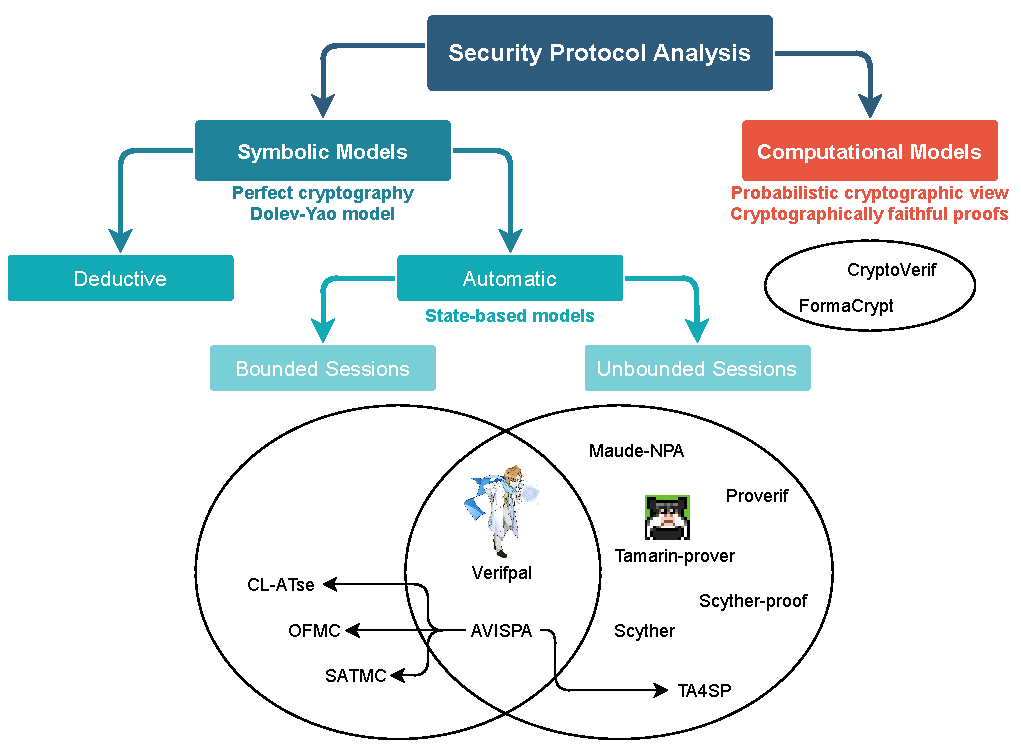
\includegraphics[scale=0.9]{symbolic-computational-model}
    \centering
    \caption{Symbolic and computational models and available tools.\\Inspired by a representation from Nicola Vitacolonna.}
    \label{fig:symbolic-computational-model}
\end{figure}

In the \textit{symbolic model} (often called Dolev-Yao model) \cite{Dolev-Yao}, the cryptographic primitives are considered as black-box and are represented using function symbols, the messages are terms and the adversary can only use defined primitives. An important aspect to note of this model is that it assumes \textbf{perfect cryptography}. As an example, consider the case in which there are two function symbols (\textbf{enc} and \textbf{dec}, used to encrypt and decrypt), a message \textit{m} and a key \textit{k} and the following equality is defined:

\begin{equation}
    \mbox{dec}\left(\mbox{enc}\left(m, k\right), k\right) = m
\end{equation}

Following from the equation $-$ and considering the perfect cryptography assumption $-$ it is possible to decrypt $\mbox{enc}\left(m, k\right)$ if and only if \textit{k} is known \cite{SymbolicComputationalBlanchet}.

In the \textit{computational model} the messages are bitstrings, the cryptographic primitives are functions from bitstrings to bitstrings, the attacker is modeled as a probabilistic Turing machine.
A security property in this model is considered to hold when the probability that it does \textit{not} hold is negligible. For instance, the previously discussed shared-key encryption can be modeled using the same equation. However, the security of encryption is expressed by stating that the attacker has an insignificant probability of breaking the primitive (e.g. decrypting the message without having the key). Security proofs using this model are usually stronger, but this comes to the cost of long, difficult, tedious, highly error-prone proofs (as stated by INRIA researchers \cite{ComputationalAnalysisCryptoSystemsINRIA}). Finally, as pointed to by Blanchet \cite{SymbolicComputationalBlanchet}, the computational model is indeed just a \textit{model} and ignores many aspects of reality and potential attacks, e.g. faulty attacks like the one affecting processors computing RSA signatures \cite{RSAFaultAttack}.

Of all the tools in \cref{fig:symbolic-computational-model}, we are going to discuss two automatic tools that employ a symbolic model: \href{https://prosecco.gforge.inria.fr/personal/bblanche/proverif/}{Proverif} and \href{https://tamarin-prover.github.io/}{Tamarin-prover}. We will also refer to Tamarin-prover as Tamarin for brevity.

We choose to focus on the tools that exploit the symbolic model as it makes it possible to automate proofs. Notice that termination is still not always guaranteed\footnote{It depends on the tool. Both Proverif and Tamarin may not terminate. Proverif proofs may end with an inconclusive result, while Tamarin will always give the correct answer (assuming termination). Other tools, like Scyther \cite{Scyther}, always terminate by limiting the growth of some parameters. More details about this problem will be discussed in \cref{sec:difficulties-analysis-symbolic}.}. From now on we will always refer to the symbolic model implicitly.

\section{Difficulties in the security protocol analysis in the symbolic model}
\label{sec:difficulties-analysis-symbolic}
Two main problems affect most automatic tools for security protocol analysis: \textbf{infinite state space} and \textbf{undecidability}.

At a high level, to verify a protocol in the symbolic model, one computes the set of terms that the adversary knows. If a certain term does not belong to this set, then the term is considered secret \cite{SymbolicVerificationBlanchet}. The difficulty is that the set of terms is infinite. Specifically, we have to deal with three sources of infinity when analyzing a protocol:
\begin{description}
    \item[\textbf{Messages}] - the adversary can produce messages of any arbitrary size;
    \item[\textbf{Sessions}] - as many attacks are possible only when multiple sessions are executed in parallel, symbolic models often use an unbounded number of sessions;
    \item[\textbf{Nonces}] - if we have an unbounded number of session, then we also must have an unbounded number of nonces to use in those sessions.
\end{description}

There have been various ways of tackling this problem:
\begin{itemize}
    \item{It is possible to decide to bound every source of infinity. In this case, the state space is finite. This method was used, for example, by Lowe \cite{LoweNeedhamSchroederPK} and SATMC \cite{SATMC};}

    \item{We can bound the number of executions of the protocol. This still leads to an infinite state space, but \cite{SymbolicModelNPCompleteInsecurity} have shown that insecurity is NP-complete;}

    \item{If we do not force any bound, the problem becomes undecidable \cite{SymbolicModelUndecidability1} \cite{SymbolicModelUndecidability2}. As pointed out by \cite{SymbolicVerificationBlanchet}, no automatic tool that always terminates and solves the problem can exist. In general, it is not possible to determine if a certain proof will, eventually, end. \Cref{fig:undecidability} shows the boundary of decidability. As evidenced by the diagram, the problem is decidable if and only if we bound at least two sources of infinity out of three.

                Of course, there are several approaches to confront this problem:

                \begin{itemize}
                    \item{Rely on help from the user. This is the approach chosen by Tamarin \cite{TamarinFoundations}, which allows for semi-automatic proofs. In Tamarin, possible resolution steps are ranked by the system, but the user can choose which to solve first;}
                    \item{Another possibility is to have tools that may return an inconclusive result $-$ yet are supposed to work correctly in most cases. Proverif follows this approach \cite{SymbolicVerificationBlanchet};}
                    \item{The last approach is to allow non-termination.}
                \end{itemize}
          }
\end{itemize}


\begin{figure}[t]
    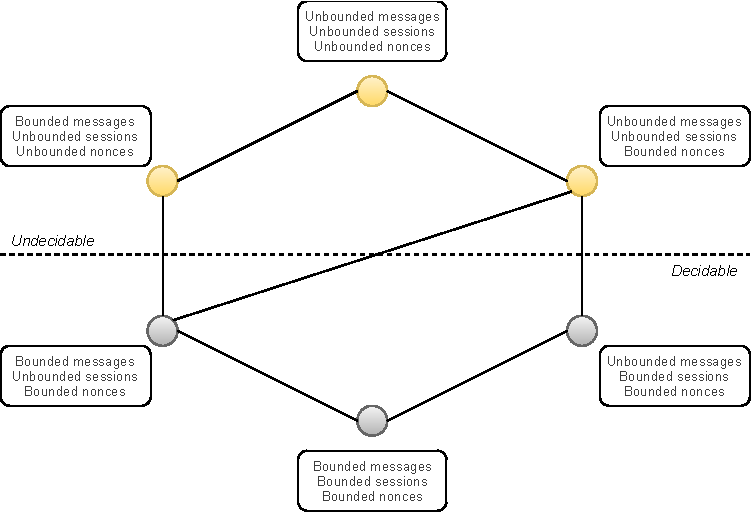
\includegraphics{undecidability}
    \centering
    \caption{Decidability of termination.\\Inspired by a representation from Nicola Vitacolonna.}
    \label{fig:undecidability}
\end{figure}

\chapter{MTProto2.0 protocol description}

In this chapter, we will give a brief overview of the MTProto2.0 protocol. A more in-depth and formal description can be found on the official web page \cite{Telegram-MTProto2.0}.

First of all, MTProto2.0 is a \textit{suite of protocols} used to enable secure communication between a Telegram client and a Telegram server over an insecure network. MTProto2.0 can be decomposed in the three following protocols:

\begin{description}[style=nextline]
    \item[Authorization] used to obtain a secret authorization key shared only with the server;
    \item[Secret-chat] used to obtain a secret key shared between two clients. This is then used to exchange end-to-end messages between two clients, with the server that basically acts as a forwarder;
    \item[Rekeying] used to achieve Perfect Forward Secrecy, allows obtaining a new end-to-end encryption key.
\end{description}

Additionally, the cloud chats encryption schema is used to securely exchange messages between clients and servers (who have shared an authorization key).

An overview on these protocols will be given in \cref{sec:auth-prot,sec:cloud-chat,sec:secret-chat,sec:rekeying}.

\section{Authorization protocol}
\label{sec:auth-prot}

%% Authorization protocol %%
\begin{figure}[!t]
\setlength{\instdist}{4cm}
\setmscoptions
\begin{msc}{}
\setmscscale{.8} 

\declinst{client}{}{Client}
\declinst{server}{}{Server}

\action*{Generates nonces $n_{c}, n_{k}$}{client}
\action*{\parbox{4.5cm}{\centering 
    Knows keys $\mbox{sk}^{(1)}, \dots, \mbox{sk}^{(n)}$\\
    Generates $n_s, g, p$\\
    Generates proof-of-work primes $q, r$
}}{server}
\nextlevel[6]

\mess{$n_{c}$}{client}{server}
\nextlevel[2]
\mess{$n_{c}, n_{s}, q \cdot r, \mbox{fp}^{(1)}, \dots, \mbox{fp}^{(n)}$}{server}{client}

\nextlevel
\action*{\parbox{4cm}{\centering
    Chooses $\mbox{pk}^{(i)}$ matching\\
    $\mbox{fp}^{(i)}$ for some $i$\\
    Factorizes $q \cdot r$\\
    $C_1 := q \cdot r, q, r, n_c, n_s, n_k$
}}{client}

\nextlevel[7]
\mess{$n_c, n_s, q, r, \mbox{fp}^{(i)}, \{\mbox{sha1}\left(C_1\right), C_1\}_{\mbox{pk}^{(i)}}$}{client}{server}
\nextlevel

\action*{$\left(k, iv\right) := \mbox{kdf}\left(n_s, n_k\right)$}{client}
\action*{\parbox{4.5cm}{\centering
    $s \in \Z_p$\\
    $g_s := g^s \mod{p}$\\
    $key, iv := \mbox{kdf}\left(n_s, n_k\right)$\\
    $S_1 := n_c, n_s, g, p, g_s, t_1$
}}{server}

\nextlevel[6]
\mess{$n_c, n_s, \left\{\mbox{sha1}\left(S_1\right), S_1\right\}_{key, iv}$}{server}{client}
\nextlevel

\action*{\parbox{4.5cm}{\centering
$c \in \Z_p$\\
$g_c := g^c \mod{p}$\\
Checks $g, p$\\
$k_{CS} := g_s^c \mod{p}$\\
$C_2 := n_c, n_s, rID, g_c$
}}{client}
\nextlevel[7]

\mess{$n_c, n_s, \left\{\mbox{sha1}\left(C_2\right), C_2\right\}_{k, iv}$}{client}{server}
\nextlevel

\action*{\parbox{4.5cm}{\centering
$k_{CS} := g_c^s \mod{p}$
}}{server}
\nextlevel[3]

\mess{$n_c, n_s, \mbox{hash}\left(n_k, k_{CS}\right)$}{server}{client}


\end{msc}
\centering
\caption{MTProto2.0 Authorization protocol}
\label{fig:authorization-protocol}
\end{figure}


The first time a Telegram client C runs the application, it must negotiate an \textbf{authorization key} with the Telegram server S. The authorization protocol is used to this end. Once the client and the server have shared an authorization key, they will use it to encrypt (almost) every future communication between them. A client might also have several keys (e.g. on multiple devices or if reinstalling the application), some of which might be locked (e.g. if the device is lost). The authorization protocol is based on the Diffie-Hellman key exchange protocol \cite{DH-protocol}.


A successful protocol run consists of three rounds, which are represented schematically in \cref{fig:authorization-protocol}:
\begin{description}
    \item[Round 1] In the first round messages are in plaintext. In particular, the client and the server exchange two nonces ($n_c$ and $n_s$). The pair $\left<n_c, n_s\right>$ identifies a session of the authorization protocol. These nonces are sent in every consequent message of the current run of the protocol, both in plaintext and encrypted form.
    \begin{enumerate}
        \item{In the first message, the client sends his fresh nonce $n_c$ to the server;}
        \item{The server answers with the client nonce $n_c$, the server fresh nonce $n_s$, a challenge $q \cdot r \leq 2^{63}$ (which are two primes used as a measure to prevent denial of service, as the client needs to spend resources on factorizing $q \cdot r$ before the server has to commit (more) resources\footnote{Notice that this might not be true as this is vulnerable to a lookup table approach (e.g. using \href{http://factordb.com}{factordb.com}).}) and a list of public RSA key fingerprints (calculated as the lower 64-bits of the SHA1 of the server public keys).}
    \end{enumerate}

    \item[Round 2] The client decomposes $q\cdot r$ in $\left<q, r\right>$, retrieves the public key of the server $pk^{\left(i\right)}$. The client then generates a nonce $n_k$ of 256 bits. This nonce $n_k$ is supposed to be secret. The pair $\left<n_s, n_k\right>$ is used, by both server and client, to derive, through a derivation function $\mbox{kdf}$, a symmetric encryption key $k$ and an initialization vector $iv$, which will be used in subsequent exchanges.
    \begin{enumerate}
        \setcounter{enumi}{2}
        \item{The client asymmetrically encrypts both $\left<q\cdot r, q, r, n_c, n_s, n_k\right>$ and its SHA1 hash with $pk^{(i)}$ and sends it along with $\left<n_c, n_s, q, r, fp^{(i)}\right>$ to the server. A rather complex padding schema is used;}
        \item{The server generates his Diffie-Hellman ephemeral key $s$ of 2048-bits, chooses $g, p$ and computes $g_s = g^s \mod{p}$. Finally, it symmetrically encrypts both $\left<n_c, n_s, g, p, g_s, t_1\right>$ and its SHA1 hash and sends it along with $\left<n_c, n_s\right>$.}
    \end{enumerate}

    Notice that the client is supposed to check that:
    \begin{itemize}
        \item{$p$ is a safe 2048-bit prime, where safe means that both $p$ and $\frac{p-1}{2}$ are prime and $2^{2047} < p < 2^{2048}$;}
        \item{$g$ is a generator for $\frac{p-1}{2}$.}
    \end{itemize}

    \item[Round 3] In the last round, the client generates his own Diffie-Hellman ephemeral key and shares it with the server.
    \begin{enumerate}
        \setcounter{enumi}{4}
        \item{The client generates his ephemeral key $c$ of 2048-bits and computes $g_c = g^c \mod{p}$. Then, it symmetrically encrypts both $\left<n_s, n_s, retryID, g_c\right>$ and its SHA1 hash and sends them along with $\left<n_c, n_s\right>$. The $retryID$ starts at zero at the time of the first attempt, otherwise is based on the values from the last failed attempt;}
        \item{The server is now able to compute the authorization key as $k_{CS} = g_c ^ s \mod{p}$. Assuming server checks pass, S sends an acknowledgment for the new key: $\left<n_c, n_s, \mbox{hash}\left(k_{CS}\right)\right>$.}
    \end{enumerate}

\end{description}

\subsection{Implementation notes}
TODO (?)








\section{Cloud-chat encryption schema}
\label{sec:cloud-chat}

%% Cloud-chat encryption schema %%
\begin{figure}[t]
    \centering
    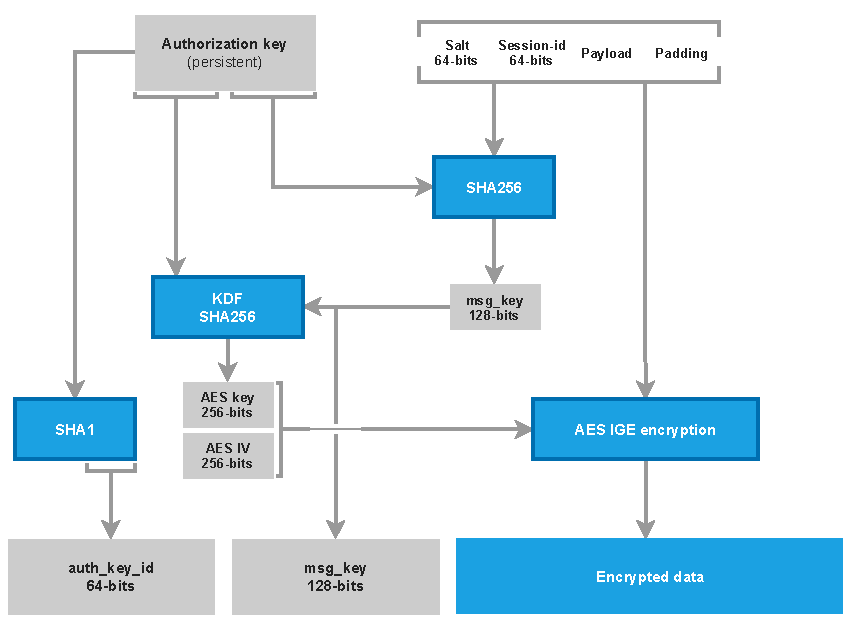
\includegraphics{cloud-chats}
    \caption{MTProto2.0 Cloud-chat protocol.\\Representation inspired by the Telegram official one.}
    \label{fig:cloud-chat-protocol}
    \end{figure}

Telegram uses the schema in \cref{fig:cloud-chat-protocol} to encrypt every message exchanged between the client and the server after an authorization key has been established using the authorization protocol in \cref{sec:auth-prot}.

A message key \textbf{msg\_key} of 128 bits is calculated as the middle 128 bits of the SHA256 of the entire message prepended by 32 bytes of the authorization key. The message itself contains a 64-bit salt, a 64-bit session id, the payload\footnote{The payload contains the time of the message, its length, a sequence number. Receiver should check these pieces of information, after decryption.} and a variable size padding of 12-1024 bytes.
The authorization key \textbf{auth\_key}, combined with the message key \textbf{msg\_key}, is used to derive a key and an initialization vector, which are used to encrypt the entire message using AES in IGE mode.

\subsection{IGE mode}
Infinite Garble Extension (in short, IGE) is a block cipher mode, lesser-known than others like ECB, CBC, OFB, CTR, CFB, GCM, CCM.
IGE can be defined with the following formula:

\begin{equation}
c_i = f_K(m_i \oplus c_{i-1}) \oplus m_{i-1}
\end{equation}

where $f_K$ stands for the encrypting function (like AES) with key $K$
and $i$ goes from 1 to $n$ $–$ the number of plaintext blocks. Two initialization vectors are also needed. \Cref{fig:IGE} summarizes how the encryption in IGE mode works.

\begin{figure}[t]
    \centering
    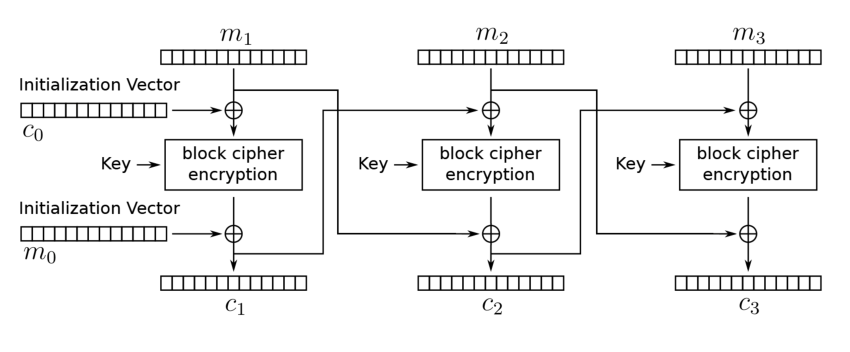
\includegraphics{IGE}
    \caption{Encryption in IGE mode.}
    \label{fig:IGE}
\end{figure}

One of the main properties of IGE mode is that it makes sure that if a ciphertext block is changed, then every subsequent block following it will not decrypt correctly.

As pointed out by \cite{Telegram-AFAQ-IGE}, the Telegram developers team is aware of the vulnerability of this mode to blockwise-adaptive Chosen Plaintext Attack (CPA)\cite{IGE-CPA}, but they claim that MTProto is not affected.




\section{Secret-chat protocol}
\label{sec:secret-chat}

%% Secret-chat protocol %%
\begin{figure}[!t]
\setlength{\instdist}{3cm}
\setmscoptions
\begin{msc}{}
\setmscscale{.8} 

\declinst{alice}{}{Alice}
\declinst{server}{}{Server}
\declinst{bob}{}{Bob}


\action*{\parbox{4.5cm}{\centering
    Knows $k_{AS}, k_{BS}$
}}{server}

\action*{\parbox{4.5cm}{\centering
    Knows $k_{AS}$
}}{alice}

\action*{\parbox{4.5cm}{\centering
    Knows $k_{BS}$
}}{bob}

\nextlevel[2]
\action*{\parbox{4.5cm}{\centering
    Gets $g, p$\\
    Generates $sid$\\
    $a \in \Z_p$\\
    $g_a := g^a \mod{p}$\\
    $M_1 := g, p, sid, g_a$
}}{alice}

\nextlevel[7]

%% TODO: Telegram webpage does not seem to specify HOW this is encrypted!!
%% UPDATE: It actually (kinda) does: it's encrypted as a cloud-chat message! For simplicity, keep this notation and explain its meaning in the written part.
\mess{$\left\{M_1\right\}_{k_{AS}}$}{alice}{server}
\nextlevel
\mess{$\left\{M_1\right\}_{k_{BS}}$}{server}{bob}

\nextlevel
\action*{\parbox{4.5cm}{\centering
    $b \in \Z_p$\\
    $g_b := g^b \mod{p}$\\
    $k_{AB} := g_a ^ b \mod{p}$\\
    $M_2 := sid, g_b, \mbox{fpk}\left(k_{AB}\right)$
}}{bob}

\nextlevel[6]
\mess{$\left\{M_2\right\}_{k_{BS}}$}{bob}{server}
\nextlevel
\mess{$\left\{M_2\right\}_{k_{AS}}$}{server}{alice}

\nextlevel
\action*{\parbox{5cm}{\centering
    $k_{AB} := g_b ^ a \mod{p}$\\
    Generates $payload$\\
    $mk := \mbox{sha256}\left(k_{AB}, payload\right)$\\
    $key, iv = \mbox{kdf}\left(k_{AB}, mk\right)$\\
    $C := \left\{payload\right\}_{key, iv}$
    $msg := \mbox{fpk}\left(k_{AB}\right), mk, C$
}}{alice}

\nextlevel[8]
\mess{$\left\{msg\right\}_{k_{AS}}$}{alice}{server}
\nextlevel
\mess{$\left\{msg\right\}_{k_{BS}}$}{server}{bob}

\end{msc}

\centering
\caption{MTProto2.0 Secret-chat protocol}
\label{fig:secret-chat-protocol}
\end{figure}

Telegram secret chats deal with end-to-end encryption between two clients (as usual, let us call the clients Alice and Bob, or A and B for brevity). After both clients have shared an authorization key with the Telegram server S, they can decide to engage themselves in a run of the secret chat protocol, allowing them to share, using a Diffie-Hellman key exchange, a shared secret. Notice that the server acts as a forwarder: every message sent from a client A to another client B is sent to the server, encrypted as a cloud chat message shown in \cref{sec:cloud-chat} with the authorization key of A; the server then decrypts the message and encrypts it as a cloud chat message using the authorization key of B and finally sends it to B. The writing $\left\{M\right\}_{k_{AS}}$ in \cref{fig:secret-chat-protocol} expresses that the message $M$ has been encrypted with the authorization key $k_{AS}$ using the cloud chat encryption schema.




\section{Rekeying protocol}
\label{sec:rekeying}

\chapter{Tools comparison}

\section{Proverif}
Let us start with a brief overview of Proverif internal reasoning. For more information, please refer to \cite{SymbolicComputationalBlanchet, SymbolicVerificationBlanchet, ProverifManual}.

\subsection{High level view}
Proverif protocols and security properties are based on an extended version of the \pic (the \textit{applied} \pic). The tool also allows the user to define constructors, destructors and equations\footnote{Destructors are basically used to de-construct some previously constructed term (e.g. decryption of an encrypted ciphertext), while equations represent term equality of some sort (e.g. commutativity of multiplication).}, which form the cryptographic primitives. The protocol is then automatically translated to a set of Horn-clauses. Using this abstract representation of the protocol (based on Horn-clauses), the Proverif verifier uses a resolution algorithm on such clauses that allows for verification of security properties \cite{SymbolicComputationalBlanchet}.
A graphical representation of the whole process is given in \cref{fig:proverif-verification-method}.

It is important to note that Proverif is not complete. This means that it may find false attacks. Moreover, it may not terminate, but it has been proven to be precise and efficient enough in practice by many case studies (the following is a non-exhaustive list of examples \cite{10.1145/1266977.1266978, ABADI20053, hal-01575923, DBLP:journals/corr/abs-2012-03141}).

We will now proceed with an overview of \pic and Horn-clauses.

\begin{figure}[t]
    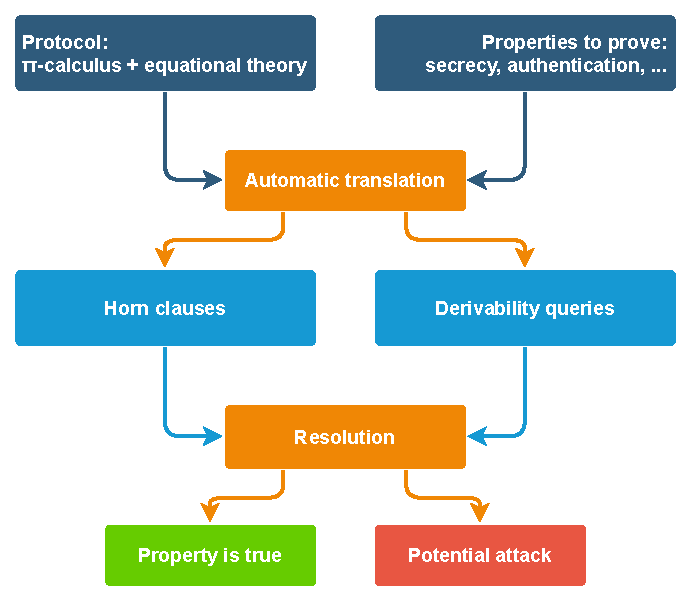
\includegraphics{proverif-verification-method}
    \centering
    \caption{Proverif verification method.\\Inspired by a representation from Bruno Blanchet \cite{SymbolicComputationalBlanchet}.}
    \label{fig:proverif-verification-method}
\end{figure}

\subsection{\pic and applied \pic}

The \pic \cite{pi-calculus-book} is a (minimal) programming that models system communicating on channels. It belongs to the \textit{process calculi} family, which is generally used to model concurrent systems. As Proverif uses the \textit{applied} \pic (which is an extension of standard \picnospace), we are going to briefly present its syntax in the rest of this section.

The following description of applied \pic references articles \cite{applied-pi-calculus-private-auth, applied-pi-calculus-abadi-1, applied-pi-calculus-abadi-2}. Please refer to these resources for further information and a more formal or in-depth description. For brevity, we only define main features of applied \pic in \cref{subsub:syntax-apic}.

\subsubsection{Overview of the syntax of the applied \pic}
\label{subsub:syntax-apic}

A \textit{signature \textSigma} is composed by a finite number of functions symbols, each with its own integer arity. Given such signature, together with an infinite set of names and an infinite set of variables, the set of \textbf{terms} is defined by the grammar:

\begin{equation}
\label{eq:apic-terms}
\begin{aligned}
    U, V &::=\\
    &a, b, \dots\\
    &x, y, \dots\\
    &f\left(U_1, \dots, U_l\right)
\end{aligned}
\qquad
\begin{aligned}
    \mbox{term}&\mbox{s}\\
    &\mbox{name}\\
    &\mbox{variable}\\
    &\mbox{constructor application}
\end{aligned}
\end{equation}

where $f \in \Sigma$ and $l$ matches the arity of $f$. Next, we define a grammar for processes, which is shown in \cref{eq:apic-processes}. As pointed to by Microsoft researchers, this grammar is very similar to the \pic \cite{applied-pi-calculus-private-auth}. We will omit defining differences from standard \pic as we have not formally defined \pic either.

\begin{equation}
\label{eq:apic-processes}
\begin{aligned}
    P, Q &::= \\
    &0 \\
    &\apicout{N}{M}{P} \\
    &\apicin{N}{x}{T}{P} \\
    &\apicpc{P}{Q}\\
    &\apicrep{P}\\
    &\apicnew{a}{T}{P}\\
    &\apicif{M}{P}{Q}
\end{aligned}
\qquad
\begin{aligned}
    \mbox{proc}&\mbox{esses} \\
    &\mbox{null process}\\
    &\mbox{output to channel N of message M}\\
    &\mbox{input from channel N of message M with sort T}\\
    &\mbox{parallel composition}\\
    &\mbox{replication}\\
    &\mbox{fresh value of sort T}\\
    &\mbox{conditional}
\end{aligned}
\end{equation}

The null process $0$ does nothing;
$\apicout{N}{M}{P}$ ($\apicin{N}{x}{T}{P}$) outputs (gets) the message M (of sort $x$) into (from) channel N and then continues with process $P$; Notice that getting a message from a channel is a blocking operation;
$\apicpc{P}{Q}$ is the parallel composition of $P$ and $Q$;
The process $\apicrep{P}$ effectively behaves as an infinite number of copies of $P$ running in parallel (\textit{unbounded} replication);
$\apicnew{a}{T}{P}$ creates a new fresh value of sort $T$, before proceeding with process $P$;
$\apicif{M}{P}{Q}$ if a standard conditional.

\comment{
$\apiclet{x}{T}{D}{P}{Q}$ is used to apply destructors or assign some term $D$ to a variable $x$ (of sort $T$);
} 



\subsection{Horn-clauses}







\section{Tamarin}
In this section we will see an overview of Tamarin foundations and internal reasoning.
For a more in-depth description and further information, see the Tamarin foundations paper \cite{TamarinFoundations} or the extended foundations paper \cite{TamarinFoundationsExtended}.

\subsection{High level view}
First of all, let us examine an high level picture of Tamarin.

The security property model of Tamarin is based on labelled multiset rewriting rules to specify protocols and adversary capabilities, a guarded fragment\footnote{Only a few examples of formulas respecting the guarded fragment of first order logic used by Tamarin will be given in \cref{sub:guarded-formulas}. See \cite{FragmentFirstOrderLogicPaper} for a rigorous definition from a mathematical point of view.} of first order logic to specify security properties\footnote{Security properties in Tamarin will also be referred to as \textit{lemmas}.} and functions and equational theories to model the algebraic properties of cryptographic protocols \cite{TamarinFoundations}.

Given the rewriting rules, security properties and equational theories, Tamarin uses a novel constraint-solving algorithm which tries to validate or falsify lemmas.

In other words, Tamarin allows to specify a labelled transition system that induces a set of traces and offers verification of such traces using a guarded fragment of first-order logic to specify ``good" traces. Tamarin then tries to prove the negation of the specified ``good" traces.

Tamarin also offers builtin equational theories \cite{TamarinProverManual}. A brief overview will be given in \cref{sub:Builtin-equational-theories}.

\subsection{Terminology}
As reported earlier, multiset rewriting rules are used to specify adversary capabilities and protocols. More precisely, a \textit{set} of \textit{labelled} multiset rewriting rules are used.

The ingredients of this multiset rewriting system are the following: 

\begin{description}[style=nextline]
    \item[Terms] which can be essentially thought of as messages. Terms can be of three different sorts. The more general sort is the \textit{msg} sort, which has two incomparable subsorts \textit{fresh} and \textit{pub} for fresh and public names, respectively;
    \item[Facts] which model information in the protocol. Facts have an arity, can be linear or persistent and are composed by terms. Linear facts model resources that can be consumed once, while persistent facts can be consumed an arbitrary number of times (and are prefixed by an exclamation mark). By convention, facts always start with a capital letter;
    \item[Special facts] Four facts are reserved and are used to model the freshness of a message $t$ ($\mbox{\textbf{Fr}}\left(t\right)$), a message $t$ coming from the public channel ($\mbox{\textbf{In}}\left(t\right)$), a message $t$ to be output to the public channel ($\mbox{\textbf{Out}}\left(t\right)$) and knowledge of a certain message $t$ from the attacker ($\mbox{\textbf{K}}\left(t\right)$);
    \item[State of the system] The state of the system is represented using a \textit{multiset} of facts;
    \item[Transition rules] A multiset of transition rules defines the possible transitions from one state to another one. Transitions are denoted with the following syntax
    \begin{equation}
        L \msrewrite{A} R
    \end{equation}
    where $L, A$ and $R$ are multisets of facts, respectively called \textbf{premises}, \textbf{actions} and \textbf{conclusions}.
    \item[Trace] A trace is a sequence $\left<A_1, \dots, A_n\right>$ of sets of ground facts denoting the sequence of actions that happened during a protocol's execution.
\end{description}


\subsection{Transition rules}
\label{sub:Transition-rules}
Let us examine an informal description of transitions.

\begin{itemize}
    \item{Let $S$ be the current state of the system}
    \item{Let $\msrnolabel{L}{R}$ be a transition rule. Note that this is a \textit{multiset rewriting rule} without a \textit{label};}
    \item{Let $\msrnolabel{l}{r}$ be a ground instance of the rule (i.e. no variables are present in the multisets);}
    \item{If we apply $\msrnolabel{l}{r}$ (assuming $l \msrsubseteq S$) to our state $S$ we reach a new state, defined by the following equation:
    \begin{equation}
        S' = S \msrsetminus l \msrcup r
    \end{equation}
    We use $\msrsetminus$, $\msrcup$ and $\msrsubseteq$ to define difference, union and subset over multisets, respectively. We can also consider the difference between linear and persistent facts and define $\lin{l}$ ($\pers{l}$) as linear facts (persistent facts) in $l$. Assuming that $\lin{l} \msrsubseteq S$ and $\pers{l} \msrsubseteq S$, then the equation becomes the following:
    \begin{equation}
        S' = S \msrsetminus \lin{l} \msrcup r
    \end{equation}
    It should be fairly clear from the equation why persistent facts can be consumed any number of times: they are never removed from the state of the system. This can be useful in scenarios in which we want to model persistent knowledge (e.g. the establishment of an encryption key $k$ may be expressed by a persistent fact $\fact{Key}{k}$).
    }
    \item{When we use labelled multiset rewriting rules, such as $\msr{l}{a}{r}$, we also add facts from $a$ to the \textit{trace} of the execution.}
\end{itemize}

\Cref{eq:builtin-tamarin-msr-rules} shows multiset rewriting rules that are always defined by Tamarin. It is not hard to see that these equations are used to model the Dolev-Yao attacker: the first rule allows the adversary to send a message $x$ he knows to someone, while the second one allows him to learn a message $x$ sent by someone.

\begin{equation}
\label{eq:builtin-tamarin-msr-rules}
\begin{gathered}
    \msr{!KU\left(x\right)}{K\left(x\right)}{In\left(x\right)}\\
    \msrnolabel{Out\left(x\right)}{\ !KD(x)}
\end{gathered}
\end{equation}


\subsection{Builtin equational theories}
\label{sub:Builtin-equational-theories}
A brief list of Tamarin built-ins is given below. Only the builtin theories considered relevant and those used in the analysis will be described here. The full list is available in the Tamarin manual. \cite{TamarinProverManual}.

\begin{description}[style=nextline]
    \item[hashing] defines a perfect hash function \textbf{h/1}\footnote{The writing \textbf{f/x} indicates that the function \textbf{f} has arity \textbf{x}.};
    \item[asymmetric-encryption] models a public key encryption scheme. It defines the following symbols:
    
    \begin{itemize}
        \item{\textbf{aenc/2}, used to model the encryption of a message with a public key}
        \item{\textbf{adec/2}, used to model the decryption of an encrypted message with a private key}
        \item{\textbf{pk/1}, used to derive a public key from a private key}
    \end{itemize}

    Functions are related by the equation \textbf{adec(aenc(msg, pk(sk)), sk) = msg};

    \item[diffie-hellman] models Diffie-Hellman groups. It defines the following symbols:
    
    \begin{itemize}
        \item{\textbf{inv/1}, models the inverse of an element}
        \item{\textbf{1/0}, models the neutral element}
        \item{\textbf{$\myexp$} and \textbf{*} symbols, models exponentiation and multiplication respectively}
    \end{itemize}

    The equational theory for this builtin is actually quite complex. For the sake of completeness, these are the related equations:
    \begin{equation}
    \begin{aligned}
        &x \myexp y \myexp z = x \myexp \left(y * z\right) \\
        &x ^ 1 = x \\
        &x * y = y * x \\
        &\left(x * y\right) * z = x * \left(y * z\right) \\
        &x * 1 = x \\
        &x * inv\left(x\right) = 1
    \end{aligned}
    \end{equation}
    % TODO: parla ancora un po' di quanto sia figo Tamarin che ha DH builtin!
\end{description}

\subsection{Guarded formulas}
\label{sub:guarded-formulas}

As reported earlier, Tamarin uses a guarded fragment of first order logic to specify security properties and $-$ in general $-$ traces. All formulas must be guarded, which essentially means that all variables quantified \textbf{must} appear in facts. \Cref{eq:guarded-formulas} shows two main formulas that respect the guarded fragment. Most $-$ if not every $-$ security property can be expressed using these formulas:

\begin{equation}
\label{eq:guarded-formulas}
\begin{gathered}
    \forall \overline{x}. F\left(\overline{z}\right) @i \Rightarrow \psi \\
    \exists \overline{x}. F\left(\overline{z}\right) @i \land \psi
\end{gathered}
\end{equation}

where $F$ is a fact, $\psi$ is guarded and $\overline{x}$ and $\overline{z}$ are vectors of terms such that $\overline{x} \subseteq \overline{z} \cup i$.
The variable $i$ is a timepoint, which annotates that the fact $F$ occurred at time $i$ (timepoints all belong to $\Q$)\footnote{Notice that timepoints are very useful to define post-compromise security properties (i.e. leaking an ephemeral key \textbf{after} honest parties have used it) and Perfect Forward Secrecy.} \cite{TamarinTeachingSlides}.

\section{Comparison of Proverif and Tamarin}
\label{section:proverif-vs-tamarin}

\comment{
    Proverif is NOT complete (see SymbolicComputationalBlanchet page 10), while Tamarin actually is (probably see foundations paper).
}

\chapter{Formalisation in Tamarin-Prover}
In this section we will dive into the implementation of the MTProto2.0 protocol created in Tamarin prover. The full code is available on github \cite{MTProto2-Tamarin}. Please refer to the README instructions for the code structure and for how to run the code.

This formalisation is based on the paper \cite{MTProto2-Proverif} and the Proverif analysis \cite{MTProto2-Proverif-impl} of MTProto2.0 by M. Miculan and N. Vitacolonna.

We will proceed analyzing the implementation of every single protocol and schema described in \cref{sec:mtproto2-informal}.

\section{Authorization protocol}
\label{sec:auth-prot-formalisation}
\subsection{Exchanges formalisation}
Let us describe, round by round, how the protocol was formalised. See \cref{fig:formalisation-authorization-protocol} for the updated schematic of the protocol.

%% Authorization protocol %%
\begin{figure}[!t]
  \setlength{\instdist}{4cm}
  \setmscoptions
  \begin{msc}{}
    \setmscscale{.8}

    \declinst{client}{}{Client}
    \declinst{server}{}{Server}

    \action*{Generates nonces $n_{c}, n_{k}$}{client}
    \action*{\parbox{4.5cm}{\centering
        Knows keys $\mbox{sk}^{(1)}, \dots, \mbox{sk}^{(n)}$\\
        Generates $n_s$
      }}{server}
    \nextlevel[4]

    \mess{$n_{c}$}{client}{server}
    \nextlevel[2]
    \mess{$n_{c}, n_{s}, \mbox{fp}^{(x)}$}{server}{client}

    \nextlevel
    \action*{\parbox{4cm}{\centering
        Gets $\mbox{pk}^{(x)}$ using $\mbox{fp}^{(x)}$\\
        $C_1 := n_c, n_s, n_k$
      }}{client}

    \nextlevel[5]
    \mess{$n_c, n_s, \mbox{fp}^{(x)}, \enc{C_1}{\mbox{pk}^{(i)}}$}{client}{server}
    \nextlevel

    \action*{$\left(k, iv\right) := \func{genKey}{n_s, n_k}$}{client}
    \action*{\parbox{4.5cm}{\centering
        $s \in \group{p}$\\
        $g_s := g^s$\\
        $key, iv := \func{genKey}{n_s, n_k}$\\
        $S_1 := n_c, n_s, g_s$
      }}{server}

    \nextlevel[6]
    \mess{$n_c, n_s, \enc{S_1}{key, iv}$}{server}{client}
    \nextlevel

    \action*{\parbox{4.5cm}{\centering
        $c \in \group{p}$\\
        $g_c := g^c$\\
        $\key{CS} := g_s^c$\\
        $C_2 := n_c, n_s, g_c$
      }}{client}
    \nextlevel[7]

    \mess{$n_c, n_s, \enc{C_2}{k, iv}$}{client}{server}
    \nextlevel

    \action*{\parbox{4.5cm}{\centering
        $\key{CS} := g_c^s$
      }}{server}
    \nextlevel[3]

    \mess{$n_c, n_s, \hash{n_k, \key{CS}}$}{server}{client}
  \end{msc}
  \centering
  \caption{MTProto2.0 Authorization protocol (simplified)}
  \label{fig:formalisation-authorization-protocol}
\end{figure}

\lstset{language=tamarin}

\paragraph{Round 1}
Client nonces (both $n_c$ and $n_k$) are generated as fresh terms.
Diffie-Hellman parameters ($p$ and $g$) are not modeled: instead, we use a single public constant \lstinline{'g'} that represents the generator. In Tamarin, this is needed to avoid having lots of partial deconstructions, a problem that causes an explosion in terms of complexity that usually leads to non-termination. As this public constant is known to everyone (including the attacker) there is no need to send it to the client in \nth{4} message. This simplification makes particularly sense if we consider that MTProto2.0 uses only six values for the generator $g$ (2, 3, 4, 5, 6 or 7).

Moreover, the proof-of-work is not used as it serves no real use for the protocol security. Finally, in our model we assume that the client has a way to get the public key of the server from its fingerprint. In Telegram, these keys are usually embedded in the application itself, resulting in the possibility of tampering \cite{MTProto2-Proverif}. Keypairs are generated using the following rule:

\begin{lstlisting}
rule RegisterPublicKey:
  let
    pkey        = pk(~skey)
    fingerprint = fpk(pkey)
  in
    [ Fr(~skey) ]
  -->
    [ !PrivateKey($X, ~skey), !PublicKey($X, pkey, fingerprint), Out(pkey) ]
\end{lstlisting}

In particular, in the model is the server who decides which public key to use and a single key fingerprint is sent to the client. As the attacker cannot add its own keys this should not matter.

\paragraph{Round 2} Another simplification is seen in the \nth{3} message: as encryption is not malleable in the symbolic model there is no need to introduce the hash of the plaintext message along with the message itself. Notice that this hash was actually used as a Message Authentication Code (MAC), which was exploited to check data integrity after decryption. This is applied to every message from now on. Public key encryption is defined using the built-in \lstinline{asymmetric-encryption} equational theory.

Time is not modeled, following from the formalisation in Proverif, and the generic key derivation function $\kdf{}$ has been renamed to $\func{genKey}{}$. Lastly, a public constant \lstinline{'StoC'} (\lstinline{'CtoS'}) has been used to mark the message from the client to the server (from the server to the client) that contains the server (client) Diffie-Hellman half key. This is needed to avoid adding an incorrect reflection attack in which the server receives the message he has previously sent. In reality, the encryption actually contains some data that allows matching messages. Symmetric encryption is modeled using the built-in \lstinline{symmetric-encryption} equational theory.

\lstset{language=tamarin}
In the implementation we also make great usage of pattern matching. Besides, the use of pattern matching is encouraged by Tamarin's manual as it usually decreases partial deconstructions. We have made use of it to ensure that half keys of client and server are actually in the form of \lstinline{'g'^~x}. This trick improves verification times by a lot, while it leaves the man-in-the-middle attack still possible\footnote{The attacker only needs to use its own ephemeral key and send the corresponding half key}.

\paragraph{Round 3} No simplification is needed for the last round, except for removing the $retryID$, meaning that we assume that the exchange is always successful. Notice that this is consistent with the MTProto2.0 specification: the client needs to retry to send his half key only when the server finds a duplicated key hash, but in our model this never happens as client and server use fresh values as Diffie-Hellman ephemeral keys, assuming correctness of the protocol.

\subsection{Additional implementation notes}
Every encrypted exchange is tagged with a public constant \lstinline{'AUTH_X'} which should result in better efficiency.

The server's nonce in the model might also be fixed. This models a flawed server implementation or a server which is lacking randomness. This is done by adding the following rules:

\begin{lstlisting}
rule GenerateRandomServerNonce:
    [ Fr(~ns) ]
  -->
    [ NS(~ns) ]

rule GenerateFixedServerNonce:
    []
  -->
    [ NS('FIXED_NS') ]
\end{lstlisting}

The server then, in the multiset rewriting rule premises, uses the \lstinline{NS(ns)} fact.

Finally, many compromise rules are created:
\begin{itemize}
  \item Compromise of server long-term key (asymmetric private key)
  \item Compromise of client secret nonce $n_k$
  \item Compromise of server ephemeral key (DH exponent)
  \item Compromise of client ephemeral key (DH exponent)
  \item Compromise of authorization keys
\end{itemize}

As compromise rules are very simple and similar to each other, we will only show an example:

\begin{lstlisting}
/* Reveals the client's DH secret exponent. */
rule CompromiseAuthProtClientExponent:
    [ !AuthProtClientEphemeralSecrets(nk, c) ]
  --[ CompromisedClientExponent(c) ]->
    [ Out(c) ]
\end{lstlisting}

Using these compromise rule, we can also check if the protocol is secure in the eCK model \cite{eCK}. The eCK model assumes, in the case of an authenticated key exchange, two parties, each having a long-term and an ephemeral secret. Of this four pieces of information, the eCK model allows to reveal any subset of these that does not contain both long-term and ephemeral secrets.
In the case of MTProto2.0, the authorization protocol does not strictly respect the eCK model as the client has no long-term secret. Moreover, intuitively, we can already notice that the protocol is not secure in the eCK model: revealing the client ephemeral secret $n_k$ allows the attacker to perform a classic man-in-the-middle attack on the Diffie-Hellman exchange \cite{MITM-DH}.

\subsection{Security properties lemmas}
Every rule in the protocol execution is labelled with action facts. We then use these to model security properties. Following the Proverif formalisation, we have modeled several forms of key agreement, authentication of parties and key secrecy, along with observational equivalence queries on the secret nonce $n_k$ and on the authorization key. In the next paragraphs we are going to examine lemmas and related results in further details.

\paragraph{Key agreement}
The following lemma models key agreement:
\begin{lstlisting}[numbers=left]
lemma LemmaAuthProtAgreement:
  "
    /* Whenever a client and a server negotiate an authorization key */
    ∀ nc ns nk authKey1 authKey2 #i #j.
      (
        ServerAcceptsAuthKey(nc, ns, nk, authKey1) @i ∧
        ClientAcceptsAuthKey(nc, ns, nk, authKey2) @j ∧

        /* and no secret was leaked */
        ¬(∃ sk #r.   CompromisedAuthKey(sk) @r) ∧
        ¬(∃ skey #r. CompromisedPrivateKey(skey) @r) ∧
        ¬(∃ n #r.    CompromisedNk(n) @r) ∧
        ¬(∃ c #r.    CompromisedClientExponent(c) @r) ∧
        ¬(∃ s #r.    CompromisedServerExponent(s) @r)
      )
      ==>
      (
        /* then the authorization key is the same */
        ( authKey1 = authKey2 ) ∨
        
        /* 
         * or the server is actually running two different instances
         * of the protocol with the client
         */
        (
          ∃ #n1 #n2.
            ServerGeneratesNonce(ns) @n1 ∧
            ServerGeneratesNonce(ns) @n2 ∧
            ¬(#n1 = #n2)
        )
      )
  "
\end{lstlisting}

By commenting any line between 10-14 (inclusive) we can model agreement in presence of some information leakage.
Key agreement without leaks holds. It may be interesting to notice that key agreement holds even when both ephemeral keys are revealed as the attacker cannot force client and server to compute different keys. Compromising one at a time either server's private key or client nonce allows the attacker to execute a man-in-the-middle attack on the Diffie-Hellman exchange.

We can also prove a similar property: if client and server end a run of the protocol negotiating the same key in their unrelated sessions, then these sessions actually coincide.

\paragraph{Authentication}
Client authentication in the protocol obviously does not hold because the client does not authenticate itself and the server is willing to execute the protocol with anybody (including the attacker). This query captures this:

\begin{lstlisting}
lemma LemmaAuthProtAuthClientToServer:
  "
    ∀ nc ns nk authKey #i #j.
      /* Whenever a client has started a session with nonce nc */
      ClientStartsSession(nc) @i ∧

      /* and the server has sent an ACK for the session <nc, ns> */
      ServerSendsAck(nc, ns, nk, authKey) @j ∧

      /* and no secret was leaked */          
      ¬(∃ sk #r.   CompromisedAuthKey(sk) @r) ∧
      ¬(∃ skey #r. CompromisedPrivateKey(skey) @r) ∧
      ¬(∃ n #r.    CompromisedNk(n) @r) ∧
      ¬(∃ c #r.    CompromisedClientExponent(c) @r) ∧
      ¬(∃ s #r.    CompromisedServerExponent(s) @r)
      ==>
      (
        /* then a client has shared an authKey with the server */
        (
          ∃ #k.
          ClientAcceptsAuthKey(nc, ns, nk, authKey) @k
        ) ∨

        /* 
         * or the server is actually running two different instances
         * of the protocol with the client
         */
        (
          ∃ #k #l.
            ServerGeneratesNonce(ns) @k ∧
            ServerGeneratesNonce(ns) @l ∧
            ¬(#k = #l)
        )
      )
  "
\end{lstlisting}

However, we can prove that the server knows for sure that the client that negotiated the authorization key is the same who sent the third message. For the sake of brevity, we will not report the related lemma.

As anyone can create an authorization key with the server, this lack of authentication is not an issue. Instead, server authentication is fundamental and it is captured by the following lemma:
\begin{lstlisting}[numbers=left]
  lemma LemmaAuthProtAuthServerToClient:
    "
      ∀ nc ns nk authKey #i1.
        /* Whenever a client receives an ACK from the server */
        ClientReceivesAck(nc, ns, nk, authKey) @i1 ∧
        
        /* and no secret was leaked */
        ¬(∃ sk #r.   CompromisedAuthKey(sk) @r) ∧
        ¬(∃ skey #r. CompromisedPrivateKey(skey) @r) ∧
        ¬(∃ n #r.    CompromisedNk(n) @r) ∧
        ¬(∃ c #r.    CompromisedClientExponent(c) @r) ∧
        ¬(∃ s #r.    CompromisedServerExponent(s) @r)
        ==>
        (
          /* then there is a session matching it on the server */
          ( 
            ∃ #j.
            ServerAcceptsAuthKey(nc, ns, nk, authKey) @j ∧
            (∀ #i2. ClientReceivesAck(nc, ns, nk, authKey) @i2 ==> #i1 = #i2)
          ) ∨

          /* or the server has reused the same nonce */
          (
            ∃ #j1 #j2.
              ServerGeneratesNonce(ns) @j1 ∧
              ServerGeneratesNonce(ns) @j2 ∧
              ¬(#j1 = #j2)
          )
        )
    "
\end{lstlisting}

This lemma holds, meaning that the server is authenticated to the client. Notice that line 19 is used to model injectivity.

\paragraph{Key secrecy}
Another fundamental property of the authentication protocol is key secrecy: when a client and a server negotiate a key, they must be sure that the key is known only to them. This property is formalised with the following lemma:
\begin{lstlisting}
lemma LemmaAuthProtKeySecrecy:
  "
    /* Whenever client and server negotiated a key */
    ∀ nc ns nk authKey #i #j #k.
      ClientAcceptsAuthKey(nc, ns, nk, authKey) @i ∧
      ServerAcceptsAuthKey(nc, nk, nk, authKey) @j ∧

      /* and the attacker knows it */
      K(authKey) @k
      ==>
      /* then some secret was leaked */
      (
        (∃ #r.      CompromisedAuthKey(authKey) @r) ∨
        (∃ skey #r. CompromisedPrivateKey(skey) @r) ∨
        (∃ #r.      CompromisedNk(nk) @r) ∨
        (∃ c #r.    CompromisedClientExponent(c) @r) ∨
        (∃ s #r.    CompromisedServerExponent(s) @r)
      )

  "
\end{lstlisting}

\paragraph{Observational equivalence}
Attempts to prove observational equivalence for client's secret nonce $n_k$ and authorization key, unfortunately, do not terminate. Notice that observational equivalence is often resources-consuming.

Observational equivalence in Tamarin is expressed using the \lstinline{diff/2} operator, which, basically, duplicates every rule, one for the left-hand side and one for the right-hand side of the operator, and tries to find a difference between the two traces.

In the formalisation, we created the two following rules:

\begin{lstlisting}
/*
 * The secret nonce nk generated by the client is indistinguishable 
 * from a fresh value.
 */
rule RuleAuthProtNkEquivalence:
    [
      !AuthProtClientEphemeralSecrets(nk, b),
      Fr(~n)
    ]
  -->
    [ Out(diff(nk, ~n)) ]

/*
 * A negotiated authorization key authKey is indistinguishable from a 
 * fresh value.
 */
rule LemmaAuthProtAuthKeyEquivalence:
    [
      !AuthKeyClient(server, authKey),
      Fr(~freshAuthKey)
    ]
  -->
    [ Out(diff(~freshAuthKey, authKey)) ]
\end{lstlisting}


\section{Cloud chat encryption schema}

\subsection{Encryption formalisation}
Cloud chat encryption has been simplified to suit the symbolic model better.
First of all, the key derivation function returns only the key. Notice that, as both key and initialization vector are derived from the same term, once the adversary is able to compute the key it would be able to compute the IV too. Hence, it is not modeled as it would only add complexity to the model without bringing any benefit.

A function \lstinline{msgKey/2} is used to create the message key from the message and the authorization key. Then, the message key is used to create the encryption key for the message, together with the authorization key, using the \lstinline{genKey/2} primitive. The plaintext message is encrypted using the built-in \lstinline{symmetric-encryption}. The final message that is sent on the channel is composed of the fingerprint of the authorization key (using \lstinline{keyID/1}), the message key and the encrypted message. Notice that functions \lstinline{msgKey/2}, \lstinline{genKey/2} and \lstinline{keyID/1} have no associated equation (i.e. are considered perfect).

Four different rules have been created: two are used to exchange messages from client to server and the other two for messages from server to client. This approach allows us to test for secrecy in both directions. Here is an example of the rule used to model a client to server message:

\begin{lstlisting}
  rule ClientCloudChatSendsMessage [color=#E2C290]:
    let
      msg = <'CC_CtoS', ~sessionID, ~m>
      mk  = msgKey(msg, authKey)
      key = genKey(mk, authKey)
      c   = <keyID(authKey), mk, senc(msg, key)>
    in
      [
        !AuthKeyClient($Server, authKey),
        Fr(~sessionID),
        Fr(~m)
      ]
    --[ ClientSendsCloudMessage(~sessionID, ~m, authKey) ]->
      [ Out(c) ]
\end{lstlisting}

Notice on line 3 that we use a public constant \lstinline{'CC_CtoS'} to differentiate client to server from server to client messages.

\subsection{Security properties lemmas}

\paragraph{Secrecy and forward secrecy} The cloud chat encryption schema is essentially employed to obtain secrecy on messages exchanges between a client and a server, after they have negotiated an authorization key.
The following lemma proves secrecy from client to server. A very similar one is used to verify secrecy of messages from server to client.

\begin{lstlisting}
lemma LemmaCloudChatSecrecyClientToServer:
  "
    /* Whenever a client sends a cloud message to the server */
    ∀ sid msg authKey #i #j #r.
      (
        ClientSendsCloudMessage(sid, msg, authKey) @i ∧

        /* and the server receives it */
        ServerReceivesCloudMessage(sid, msg, authKey) @j ∧

        /* and the attacker knows it */
        K(msg) @r
      )
      ==>
      (
        /* then some secret was compromised */
        (∃ #r.      CompromisedAuthKey(authKey) @r) ∨
        (∃ skey #r. CompromisedPrivateKey(skey) @r) ∨
        (∃ n #r.    CompromisedNk(n) @r) ∨
        (∃ c #r.    CompromisedClientExponent(c) @r) ∨
        (∃ s #r.    CompromisedServerExponent(s) @r)
      )
  "
\end{lstlisting}

This lemma actually means that messages are secure, unless:
\begin{itemize}
  \item The private key of the server is compromised
  \item The secret nonce $n_k$ of the client is compromised
  \item Diffie-Hellman exponents of client or server
\end{itemize}

As seen in \cref{sec:auth-prot-formalisation}, compromising any of these secrets leads to a lack of secrecy on they key. Additionally, also che compromise key itself can be compromised to break cloud chat secrecy.

Notice that this means that perfect forward secrecy does not hold in cloud chats as an attacker that is able to compromise the authorization key can decrypt both past and future messages (as well as forging them, impersonating the client to the server).

\chapter{Comparison with Proverif}
\input{./chapters/06_comparison}

%% Fine dei capitoli normali, inizio dei capitoli-appendice (opzionali)
% \appendix

%% Parte conclusiva del documento; tipicamente per riassunto, bibliografia e/o indice analitico.
\backmatter

%% Riassunto (opzionale)
%\summary

%% Bibliografia (praticamente obbligatoria)
\bibliographystyle{plain_\languagename}
\bibliography{thud}

\end{document}